\documentclass{evolang12}
\usepackage{graphicx}
\usepackage{url}
\usepackage{authblk}


\begin{document}


\title{Lexicalization of conceptual hierarchies \\ through communicative interaction}
\author[1*]{ANONYMOUS AUTHOR 1}
\author[1]{ANONYMOUS AUTHOR 2} 
\author[2]{ANONYMOUS AUTHOR 3}
\author[3]{ANONYMOUS AUTHOR 4}
\affil[*]{Corresponding Author: name@domain.com}
\affil[1]{This Department, University X, City, Country}
\affil[2]{That Department, University Y, City, Country}
\affil[3]{Other Department, University Z, City, Country}

%%%%% INSTRUCTIONS FOR ADDING AUTHORS %%%%%

%Initial submissions should be anonymous - DO NOT INCLUDE ANY IDENTIFYING INFORMAITON IN THE SUBMISSION VERSION -(i.e., no author details should be added above). To avoid problems with page limits, please include the appropriate number of placeholders for authors. If multiple authors share an affiliation, they can be paired with the appropriate affiliation using the numbers in the square brackets next to "author" and "affil" to save space. Designate a single corresponding author using the asterisk.

\maketitle

%% Introduce problem
Natural languages provide speakers with remarkable flexibility in their choice of referring expressions. In addition to the combinatorial explosion of possible modifiers afforded by compositional semantics \cite{Partee95_LexicalSemanticsCompositionality,VanDeemterEtAl12_ReferenceProduction,WintersKirbySmith14_LanguagesAdapt}, we have a number of lexicalized nominal terms at our disposal. \emph{Dalmatian}, \emph{dog}, and \emph{animal} can all truthfully be used to talk about the same Dalmatian at different levels of specificity, with one level of the hierarchy -- the \emph{basic-level} -- privileged over the others \cite{RoschMervisGray___BoyesBraem76_BasicObjects}. Recent work has investigated the synchronic pragmatics of nominal reference across different contexts, explaining the basic-level bias in terms of informativeness and production cost \cite<e.g.>{GrafEtAl16_BasicLevel}. But there remains a more fundamental evolutionary question: why do multiple levels of reference coexist in the lexicon instead of a simpler system only containing subordinate terms? And what gives rise to a distinguished basic-level?

%% Introduce hypothesis & interactive paradigm
Our hypothesis, motivated both by classic work on concept representations and contemporary work on the selective pressures induced by communication, is that lexicalization of conceptual hierarchies is a function of (1) the structure and statistics of entities in the environment, and (2) the particular contexts in which communication occurs. In particular, we expect hierarchical lexica to form when features can be encoded as predictable clusters and communicative goals require distinctions to be drawn at multiple levels. To test this hypothesis, we designed a repeated reference game in which pairs of participants interactively created an artificial language to communicate with each other about objects in context. 

%% Introduce task 
In this game, participants were paired over the web and placed in a shared environment containing a grid of four objects and a `chatbox' to send messages from a pre-specified vocabulary of sixteen words (Fig. 1A). On each of ninety trials, one player --- the `speaker' --- was privately shown a highlighted target object and allowed to send a single word to help their partner select this object from the array of distractors. The set of objects was designed to cluster in a natural hierarchy so that distractors could either belong to the same subordinate-, basic-, or super-ordinate level as the target. In addition to fine-grained behavioral trajectories observed over the course of the game, we conducted a lexicalization post-test in which each player gave explicit judgements about the meaning of each word by selecting all objects to which that word applies. %Players were awarded bonuses for correct responses and switched roles on each round for a total of 90 rounds. Neither player was trained on word-object mappings in advance, so all meanings had to be created over the course of interaction. 

%% Introduce manipulations & summarize results; suggest interpretation (i.e. path-dependence?) and speculate about set-based version & model?

We manipulated the statistics of the context in a between-subjects design to test the contribution of communicative relevance to lexicalization. In the critical `uniform' condition, distractors were equally likely to appear at any level of the hierarchy. We also ran three control conditions in which the majority of trials had distractors at only one level, e.g. in the `subordinate-majority' condition, the majority of trials had competitors at the subordinate level, theoretically requiring speakers to lexicalize a label for each target. We found that only the uniform condition systematically gave rise to lexica in which multiple levels of reference coexist (see Fig. 1B). This suggests that pragmatic pressures for informativity in a diversity of communicative contexts is instrumental for the lexicalization of hierarchical nominal reference systems. 


\begin{figure}[t]
\begin{center}
\scalebox{0.4}{
  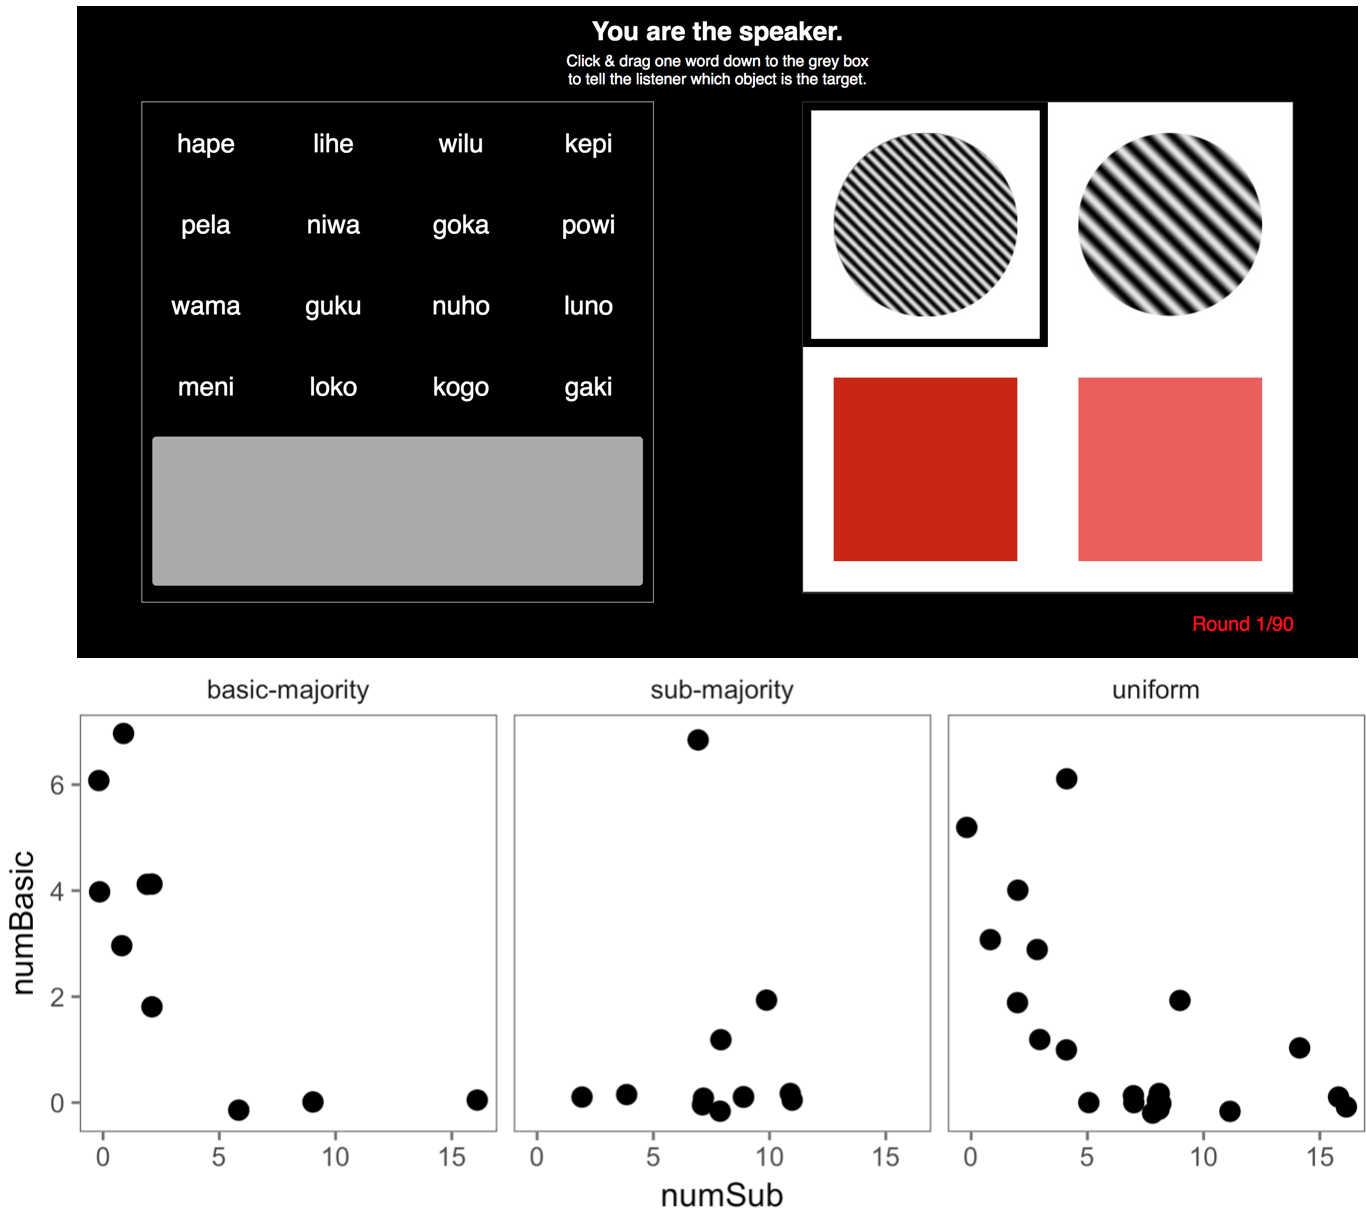
\includegraphics{fig.png}
}
\end{center}
\caption{{\footnotesize (A) Example round from experiment in subordinate-required condition; (B) results \label{exp}}}
\end{figure}

\bibliographystyle{apacite}
\bibliography{evolang} 

\end{document}
